% =========================================================
%  ppt/11-level-physics-kontrol.tex
%  Materi 11 — Membangun Level, Physics, dan Kontrol Pemain
%  Bab XIII buku ajar
% =========================================================
\documentclass[aspectratio=169,10pt]{beamer}
% =========================================================
%  ppt/config/packages.tex
%  Paket bersama untuk seluruh presentasi kuliah
%  Pengantar Pemrograman Game
% =========================================================

\usepackage[T1]{fontenc}
\usepackage[utf8]{inputenc}
\usepackage[indonesian]{babel}
\usepackage{lmodern}
\usepackage{textcomp}
\usepackage{amsmath}
\usepackage{amssymb}
\usepackage{graphicx}
\usepackage{booktabs}
\usepackage{tabularx}
\usepackage{array}
\usepackage{multicol}
\usepackage{listings}
\usepackage{upquote}
\usepackage{adjustbox}
\usepackage{tcolorbox}
\usepackage{tikz}
\usetikzlibrary{
  arrows.meta,
  positioning,
  shapes.geometric,
  shapes.misc,
  calc,
  fit,
  backgrounds,
  matrix,
  chains,
  decorations.pathreplacing,
  patterns
}

\tcbuselibrary{skins}

% Jangan memuat geometry: ukuran halaman diatur oleh beamer.

% =========================================================
%  ppt/config/theme.tex
%  Satu tema Beamer untuk keempat belas presentasi
%  Pengantar Pemrograman Game
% =========================================================

% --------------------------------------------------------- warna
\definecolor{ubNavy}{HTML}{1F3864}
\definecolor{ubAccent}{HTML}{2E75B6}
\definecolor{ubHead}{HTML}{D9E2F3}
\definecolor{ubSoft}{HTML}{F2F6FC}
\definecolor{ubLine}{HTML}{BFBFBF}
\definecolor{ubText}{HTML}{1F2937}
\definecolor{ubMuted}{HTML}{5A6678}
\definecolor{ubGreen}{HTML}{1E7B45}
\definecolor{ubGreenBg}{HTML}{F1F8F2}
\definecolor{ubRed}{HTML}{B3261E}
\definecolor{ubRedBg}{HTML}{FDF2F1}
\definecolor{ubWarn}{HTML}{A35A05}
\definecolor{ubWarnBg}{HTML}{FFF8EC}
\definecolor{ubGray}{HTML}{F6F6F6}
\definecolor{ubCodeBg}{HTML}{10233F}
\definecolor{ubCodeText}{HTML}{E8EEF7}
\definecolor{ubCodeKey}{HTML}{8FBCF0}
\definecolor{ubCodeCom}{HTML}{8FB37A}
\definecolor{ubCodeStr}{HTML}{D9A46B}
\definecolor{ubCodeNum}{HTML}{7E99BE}

% Nama warna yang dipakai gambar TikZ buku ajar.
\definecolor{ubPrimary}{HTML}{1F3864}
\definecolor{ubAlt}{HTML}{F2F6FC}

% --------------------------------------------------------- dasar
\usetheme{default}
\usefonttheme{professionalfonts}
\setbeamertemplate{navigation symbols}{}
\setbeamerfont{frametitle}{size=\Large,series=\bfseries}
\setbeamerfont{framesubtitle}{size=\small}
\setbeamerfont{footline}{size=\tiny}
\setbeamerfont{block title}{size=\small,series=\bfseries}
\setbeamerfont{block body}{size=\small}
\setbeamerfont{itemize/enumerate body}{size=\small}
\setbeamerfont{itemize/enumerate subbody}{size=\footnotesize}

\setbeamersize{text margin left=0.60cm,text margin right=0.60cm}
\uchyph=0

\setbeamercolor{normal text}{fg=ubText,bg=white}
\setbeamercolor{structure}{fg=ubAccent}
\setbeamercolor{frametitle}{fg=ubNavy,bg=white}
\setbeamercolor{title}{fg=ubNavy}
\setbeamercolor{footline}{fg=ubMuted,bg=white}
\setbeamercolor{itemize item}{fg=ubAccent}
\setbeamercolor{itemize subitem}{fg=ubAccent}
\setbeamercolor{block title}{fg=white,bg=ubNavy}
\setbeamercolor{block body}{fg=ubText,bg=ubSoft}
\setbeamercolor{block title alerted}{fg=white,bg=ubWarn}
\setbeamercolor{block body alerted}{fg=ubText,bg=ubWarnBg}
\setbeamercolor{block title example}{fg=white,bg=ubGreen}
\setbeamercolor{block body example}{fg=ubText,bg=ubGreenBg}
\setbeamercolor{caption name}{fg=ubMuted}

\setbeamertemplate{blocks}[rounded][shadow=false]
\setbeamertemplate{itemize item}{\raisebox{0.10em}{\color{ubAccent}\scriptsize$\blacksquare$}}
\setbeamertemplate{itemize subitem}{\raisebox{0.06em}{\color{ubAccent}\tiny$\blacktriangleright$}}
\setbeamertemplate{enumerate item}{%
  \makebox[1.3em][l]{\color{ubAccent}\insertenumlabel.}}

\addtobeamertemplate{itemize/enumerate body begin}{%
  \setlength{\itemsep}{0.42em}\setlength{\parskip}{0pt}}{}

% --------------------------------------------------------- judul frame
\setbeamertemplate{frametitle}[default][left]

% --------------------------------------------------------- kaki
\newcommand{\materino}{00}
\newcommand{\materifoot}{Pengantar Pemrograman Game \textperiodcentered\ Materi \materino}

\setbeamertemplate{footline}{%
  \begin{beamercolorbox}[wd=\paperwidth,ht=0.015cm,dp=0cm]{footline}%
    \color{ubHead}\rule{\paperwidth}{0.4pt}%
  \end{beamercolorbox}%
  \begin{beamercolorbox}[wd=\paperwidth,ht=0.40cm,dp=0.14cm,%
                         leftskip=0.60cm,rightskip=0.60cm]{footline}%
    \usebeamerfont{footline}\color{ubMuted}\materifoot\hfill\insertframenumber%
  \end{beamercolorbox}%
}

% --------------------------------------------------------- makro buku ajar
\providecommand{\code}[1]{\texttt{\detokenize{#1}}}
\providecommand{\istilah}[1]{\emph{#1}}
\providecommand{\CPMK}[1]{CPMK\,#1}
\providecommand{\CPL}[1]{CPL\,#1}
\providecommand{\SUBCPMK}[1]{Sub-CPMK\,#1}

% --------------------------------------------------------- gaya kode
\lstdefinelanguage{CSharp}{
  morekeywords={abstract,as,base,bool,break,byte,case,catch,char,class,const,
    continue,decimal,default,delegate,do,double,else,enum,event,explicit,
    extern,false,finally,fixed,float,for,foreach,goto,if,implicit,in,int,
    interface,internal,is,lock,long,namespace,new,null,object,operator,out,
    override,params,private,protected,public,readonly,ref,return,sbyte,
    sealed,short,sizeof,stackalloc,static,string,struct,switch,this,throw,
    true,try,typeof,uint,ulong,unchecked,unsafe,ushort,using,virtual,void,
    volatile,while,var,get,set},
  sensitive=true,
  morecomment=[l]{//},
  morecomment=[s]{/*}{*/},
  morestring=[b]",
}

\lstdefinestyle{kode}{
  basicstyle=\ttfamily\footnotesize\color{ubCodeText},
  keywordstyle=\color{ubCodeKey}\bfseries,
  commentstyle=\color{ubCodeCom}\itshape,
  stringstyle=\color{ubCodeStr},
  numberstyle=\tiny\color{ubCodeNum},
  numbers=left,
  numbersep=7pt,
  backgroundcolor=\color{ubCodeBg},
  frame=none,
  showstringspaces=false,
  breaklines=false,
  tabsize=4,
  columns=fullflexible,
  keepspaces=true,
  xleftmargin=12pt,
  xrightmargin=2pt,
  aboveskip=0pt,
  belowskip=0pt,
  upquote=true,
}
\lstset{style=kode}

\newcommand{\kodejelas}[1]{%
  \vspace{0.16cm}%
  {\footnotesize\color{ubMuted}#1\par}%
}
\newcommand{\sumber}[1]{%
  \vspace{0.08cm}%
  {\scriptsize\color{ubMuted}\itshape #1\par}%
}
\newcommand{\awalan}[1]{%
  {\small\color{ubMuted}#1\par}\vspace{0.18cm}%
}

% --------------------------------------------------------- kotak
\newtcolorbox{kotak}[1][]{enhanced, colback=ubSoft, colframe=ubAccent,
  boxrule=0pt, leftrule=2.2pt, arc=1pt, left=6pt, right=6pt, top=4pt,
  bottom=4pt, fontupper=\footnotesize, #1}
\newtcolorbox{peringatan}[1][]{enhanced, colback=ubWarnBg, colframe=ubWarn,
  boxrule=0pt, leftrule=2.2pt, arc=1pt, left=6pt, right=6pt, top=4pt,
  bottom=4pt, fontupper=\footnotesize, #1}
\newtcolorbox{kiat}[1][]{enhanced, colback=ubGreenBg, colframe=ubGreen,
  boxrule=0pt, leftrule=2.2pt, arc=1pt, left=6pt, right=6pt, top=4pt,
  bottom=4pt, fontupper=\footnotesize, #1}

% --------------------------------------------------------- sampul
% \deckcover{nomor}{minggu}{judul}{sub-cpmk}{teknologi}{sumber}{blok}
\newcommand{\deckcover}[7]{%
\begin{frame}[plain]
\begin{tikzpicture}[remember picture, overlay]
  \fill[ubNavy] (current page.south west) rectangle ([xshift=6.00cm]current page.north west);
  \fill[ubAccent] ([xshift=6.00cm]current page.south west) rectangle ([xshift=6.08cm]current page.north west);

  \node[anchor=north west, text width=4.72cm, align=left, inner sep=0pt]
    at ($(current page.north west)+(0.66cm,-0.60cm)$) {%
      {\color{white}\bfseries\fontsize{10.2}{12.2}\selectfont
       Universitas Bale Bandung}\\[4pt]
      {\color{ubHead}\fontsize{7.6}{9.4}\selectfont
       Fakultas Teknologi Informasi}\\[1pt]
      {\color{ubHead}\fontsize{7.6}{9.4}\selectfont
       Program Studi Teknik Informatika}\\[7pt]
      {\color{ubAccent}\rule{4.0cm}{0.5pt}}%
    };

  \node[anchor=north west, text width=4.72cm, align=left, inner sep=0pt]
    at ($(current page.north west)+(0.66cm,-2.72cm)$) {%
      {\color{ubAccent}\fontsize{6.4}{7.8}\selectfont MATA KULIAH}\\[3pt]
      {\color{white}\bfseries\fontsize{9.8}{12.0}\selectfont
       Pengantar Pemrograman Game}\\[3pt]
      {\color{ubHead}\fontsize{7.6}{9.4}\selectfont
       MWCA009 \textperiodcentered\ 3 SKS}\\[8pt]
      {\color{ubHead}\fontsize{7.6}{9.4}\selectfont
       Semester Ganjil 2026/2027}%
    };

  \node[anchor=south west, text width=4.72cm, align=left, inner sep=0pt]
    at ($(current page.south west)+(0.66cm,0.52cm)$) {%
      {\color{ubAccent}\fontsize{6.4}{7.8}\selectfont DOSEN PENGAMPU}\\[3pt]
      {\color{white}\fontsize{8.4}{10.4}\selectfont
       Cecep Suwanda, S.Si., M.Kom.}%
    };

  \node[anchor=north west, text width=8.95cm, align=left, inner sep=0pt]
    at ($(current page.north east)+(-9.40cm,-0.92cm)$) {%
      {\color{ubAccent}\bfseries\fontsize{8.2}{10.2}\selectfont
       MATERI #1\ \ \textperiodcentered\ \ MINGGU #2}\\[8pt]
      {\color{ubNavy}\bfseries\fontsize{19.4}{23.4}\selectfont
       \hyphenpenalty=10000 \exhyphenpenalty=10000 \raggedright #3}%
    };

  \node[anchor=north west, text width=8.95cm, align=left, inner sep=0pt]
    at ($(current page.north east)+(-9.40cm,-4.30cm)$) {%
      \renewcommand{\arraystretch}{1.30}%
      \begin{tabular}{@{}>{\color{ubMuted}\fontsize{7.3}{9.0}\selectfont}p{1.85cm}
                        >{\color{ubText}\fontsize{8.1}{10.0}\selectfont}p{6.7cm}@{}}
        Sub-CPMK      & #4 \\
        Teknologi     & #5 \\
        Sumber materi & #6 \\
        Blok          & #7 \\
      \end{tabular}%
    };
\end{tikzpicture}
\end{frame}%
}

% --------------------------------------------------------- pembatas bagian
\newcommand{\sectionframe}[3]{%
\begin{frame}[plain]
\begin{tikzpicture}[remember picture, overlay]
  \fill[ubNavy] (current page.south west) rectangle (current page.north east);
  \fill[ubAccent] (current page.north west) rectangle ([xshift=0.10cm]current page.south west);
  \node[anchor=west, inner sep=0pt]
    at ($(current page.west)+(1.00cm,1.45cm)$)
    {\color{ubNavy!52!white}\bfseries\fontsize{58}{58}\selectfont #1};
  \node[anchor=west, inner sep=0pt, text width=11.6cm, align=left]
    at ($(current page.west)+(1.05cm,-0.55cm)$) {%
      {\color{ubAccent}\bfseries\fontsize{8.0}{10.0}\selectfont BAGIAN}\\[3pt]
      {\color{white}\bfseries\fontsize{20.5}{24.5}\selectfont #2}\\[5pt]
      {\color{ubHead}\small #3}%
    };
  \node[anchor=south east, inner sep=0pt]
    at ($(current page.south east)+(-0.60cm,0.32cm)$)
    {\color{ubHead}\fontsize{7.4}{9}\selectfont #1 / 6
     \ \ \textperiodcentered\ \ \insertframenumber};
\end{tikzpicture}
\end{frame}%
}

% --------------------------------------------------------- peta pertemuan
\newcommand{\blokpeta}[6]{%
  \ifnum#2=#3
    \node[rounded corners=3pt, fill=ubNavy, draw=ubNavy, line width=0.5pt,
          text width=3.02cm, minimum height=1.62cm, align=left, inner sep=5pt]
      at (#1,0) {%
        {\color{ubAccent}\bfseries\fontsize{6.8}{8}\selectfont #4}\\[1pt]
        {\color{white}\bfseries\fontsize{7.6}{9}\selectfont #5}\\[2pt]
        {\color{ubHead}\fontsize{6.4}{7.6}\selectfont #6}};
  \else
    \node[rounded corners=3pt, fill=ubSoft, draw=ubHead, line width=0.5pt,
          text width=3.02cm, minimum height=1.62cm, align=left, inner sep=5pt]
      at (#1,0) {%
        {\color{ubAccent}\bfseries\fontsize{6.8}{8}\selectfont #4}\\[1pt]
        {\color{ubNavy}\bfseries\fontsize{7.6}{9}\selectfont #5}\\[2pt]
        {\color{ubMuted}\fontsize{6.4}{7.6}\selectfont #6}};
  \fi
}

% \petapertemuan{blok aktif}{sebelumnya}{sesudahnya}{keluaran}
% \petapertemuan{blok aktif}{sebelumnya}{pertemuan ini}{sesudahnya}{keluaran}
\newcommand{\petapertemuan}[5]{%
\begin{frame}{Peta Pertemuan}
{\scriptsize\color{ubMuted}Kedudukan materi dalam empat blok perkuliahan}\par
\vspace{0.10cm}
\centering
\begin{tikzpicture}
  \blokpeta{-5.58}{1}{#1}{BLOK I}{Materi 1--5}{Game loop, vektor,\\fisika, collision}
  \blokpeta{-1.86}{2}{#1}{BLOK II}{Materi 6--9}{AI NPC: chase, FSM,\\pathfinding A*}
  \blokpeta{1.86}{3}{#1}{BLOK III}{Materi 10--11}{Unity: scene,\\level, physics}
  \blokpeta{5.58}{4}{#1}{BLOK IV}{Materi 12--14}{Aset visual, audio,\\UI, playtest}
\end{tikzpicture}
\par\vspace{0.30cm}
\begin{columns}[T,onlytextwidth]
  \begin{column}{0.315\textwidth}
    \begin{beamercolorbox}[wd=\linewidth,sep=4pt,rounded=true]{block body}
      {\color{ubMuted}\fontsize{6.6}{8}\selectfont SEBELUMNYA}\\[2pt]
      {\footnotesize #2}
    \end{beamercolorbox}
  \end{column}
  \begin{column}{0.315\textwidth}
    \begin{beamercolorbox}[wd=\linewidth,sep=4pt,rounded=true]{block title}
      {\color{ubHead}\fontsize{6.6}{8}\selectfont PERTEMUAN INI}\\[2pt]
      {\footnotesize #3}
    \end{beamercolorbox}
  \end{column}
  \begin{column}{0.315\textwidth}
    \begin{beamercolorbox}[wd=\linewidth,sep=4pt,rounded=true]{block body}
      {\color{ubMuted}\fontsize{6.6}{8}\selectfont SESUDAHNYA}\\[2pt]
      {\footnotesize #4}
    \end{beamercolorbox}
  \end{column}
\end{columns}
\par\vspace{0.26cm}
{\footnotesize\color{ubText}\textbf{Keluaran pertemuan.} #5\par}
\end{frame}%
}

% --------------------------------------------------------- penutup
\newcommand{\penutup}[2]{%
\begin{frame}[plain]
\begin{tikzpicture}[remember picture, overlay]
  \fill[ubNavy] (current page.south west) rectangle (current page.north east);
  \fill[ubAccent] (current page.north west) rectangle ([xshift=0.10cm]current page.south west);

  \node[anchor=north west, text width=13.6cm, align=left, inner sep=0pt]
    at ($(current page.north west)+(1.00cm,-0.95cm)$) {%
      {\color{ubAccent}\bfseries\fontsize{8.2}{10}\selectfont ASESMEN MINGGU INI}\\[6pt]
      {\color{white}\bfseries\fontsize{24}{28}\selectfont #1}%
    };

  \node[anchor=north west, text width=13.6cm, align=left, inner sep=0pt]
    at ($(current page.north west)+(1.00cm,-4.55cm)$) {%
      {\color{ubNavy!0!ubHead}\rule{13.4cm}{0.4pt}}\\[7pt]
      {\color{ubAccent}\bfseries\fontsize{7.4}{9}\selectfont
       PENGAIT KE MATERI BERIKUTNYA}\\[4pt]
      {\color{ubHead}\fontsize{10.6}{13.2}\selectfont #2}%
    };

  \node[anchor=south east, inner sep=0pt]
    at ($(current page.south east)+(-0.60cm,0.32cm)$)
    {\color{ubHead}\fontsize{7.4}{9}\selectfont \insertframenumber};
\end{tikzpicture}
\end{frame}%
}



\renewcommand{\materino}{11}

\begin{document}

\deckcover{11}{12}
  {Membangun Level, Physics, dan Kontrol Pemain}
  {3.2}
  {Unity}
  {Bab XIII buku ajar}
  {Blok III \textperiodcentered\ Materi 10--11}

% --------------------------------------------------------- capaian
\begin{frame}{Capaian Pertemuan}
\setbeamerfont{itemize/enumerate body}{size=\scriptsize}
\awalan{Sub-CPMK dan indikator dari RPS, serta tujuan Bab XIII buku ajar.}
\begin{columns}[T,onlytextwidth]
  \begin{column}{0.52\textwidth}
    \begin{beamercolorbox}[wd=\linewidth,sep=5pt,rounded=true]{block title}
      {\fontsize{6.8}{8}\selectfont\color{ubHead}SUB-CPMK 3.2 \textperiodcentered\ RANAH C4}\\[2pt]
      {\footnotesize Membangun level 2D/3D sederhana dengan \emph{collider},
       \emph{Rigidbody}, dan kontrol pemain.}
    \end{beamercolorbox}
    \vspace{0.14cm}

    {\fontsize{7}{8.5}\selectfont\bfseries\color{ubAccent}INDIKATOR}\par
    \vspace{0.06cm}
    \begin{itemize}
      \item Menyusun level menggunakan \emph{tilemap}/\emph{greyboxing}.
      \item Mengonfigurasi Collider dan Rigidbody sesuai kebutuhan mekanik.
      \item Menganalisis dan memperbaiki masalah fisika: \emph{jitter}, objek
            menembus Collider, dan jatuh tanpa henti.
    \end{itemize}
    \vspace{0.10cm}
    \begin{kotak}
      Bab ini menutup CPMK 3. Indikator ketiga menuntut ranah C4: bukan sekadar
      memasang komponen, melainkan menelusuri gejala sampai penyebabnya.
    \end{kotak}
  \end{column}
  \begin{column}{0.45\textwidth}
    {\fontsize{7}{8.5}\selectfont\bfseries\color{ubAccent}TUJUAN BAB XIII}\par
    \vspace{0.08cm}
    \begin{itemize}
      \item Menyusun level secara greyboxing dan dengan tilemap.
      \item Memilih antara Collider biasa dan \emph{trigger volume}, beserta
            akibat pilihannya.
      \item Menjelaskan tiga tipe Rigidbody dan menentukan tipe yang tepat.
      \item Menulis kontrol pemain yang menggerakkan Rigidbody pada
            \emph{FixedUpdate}, beserta pemeriksaan tanah.
      \item Menjelaskan mengapa masukan dibaca pada Update sedangkan gerak
            dikerjakan pada FixedUpdate.
      \item Menganalisis dan memperbaiki empat masalah fisika.
    \end{itemize}
  \end{column}
\end{columns}
\end{frame}

% --------------------------------------------------------- peta
\petapertemuan{3}
  {Materi 10 \textperiodcentered\ Pengenalan Unity: \emph{Project},
   \emph{Scene}, dan \emph{GameObject}}
  {Materi 11 \textperiodcentered\ Membangun Level, \emph{Physics}, dan Kontrol
   Pemain}
  {Materi 12 \textperiodcentered\ Impor Aset Visual, Animasi, dan UI Dasar}
  {Level Unity yang dapat dimainkan: pemain berjalan, melompat, mendarat,
   dan terhalang; daerah trigger memanggil fungsinya; catatan perbaikan
   masalah fisika.}

% ========================================================= bagian 1
\section{Menyusun Level}
\sectionframe{01}{Menyusun Level}
  {Dari balok abu-abu menjadi ruang yang dapat diuji}

\begin{frame}{Greyboxing: Menguji Mekanik Sebelum Aset}
\awalan{Level pertama disusun dari balok abu-abu tanpa tekstur, tanpa warna, dan
tanpa aset. Cara itu disebut \emph{greyboxing}.}
\begin{itemize}
  \item Tujuannya bukan keindahan, melainkan \textbf{menguji mekanik}
        permainan sebelum aset yang mahal dibuat.
  \item Mengubah susunan balok jauh lebih murah daripada mengubah aset yang
        sudah dibuat sesuai susunan lama.
  \item Bila jalur ternyata terlalu sempit atau lompatannya terlalu jauh, yang
        perlu diubah hanyalah letak beberapa balok.
  \item Kotak kuning yang ditampilkan mesin adalah bentuk batas benda: itulah
        yang diperiksa untuk tabrakan, bukan bentuk yang dilihat pemain.
\end{itemize}
\begin{kotak}
Sebelum menyusun level panjang, buat satu ruang kecil (\emph{gym} atau
\emph{test level}) yang memuat seluruh mekanik yang direncanakan: satu
lompatan, satu rintangan, dan satu benda yang dapat dipungut.
\end{kotak}
\end{frame}

\begin{frame}{Menyusun Level dengan Tilemap}
\awalan{Level dua dimensi yang petaknya berulang---lantai dan dinding---dapat
disusun dengan \emph{tilemap}.}
\begin{itemize}
  \item \emph{Tilemap} adalah lembaran petak yang dapat diisi dengan pola.
  \item Ia tersusun atas dua hal: \texttt{Tilemap} sebagai lembarannya dan
        \texttt{Tilemap Collider 2D} sebagai bentuk batasnya.
  \item Seluruh petak yang tersusun hanya memerlukan satu Collider, sehingga
        jauh lebih ringan daripada susunan balok yang sama banyaknya.
  \item Ukuran ditetapkan lebih dahulu, dalam meter: tinggi lompatan pemain,
        lebar celah yang dapat dilewati, dan tinggi bongkahan.
  \item Ketiganya saling bergantung: bila tinggi lompatan 2,5 meter, celah
        setinggi 3 meter mustahil dilewati.
\end{itemize}
\begin{kotak}
Susun level agar seluruh celahnya terjangkau, dengan menyisakan kelonggaran
sekitar sepuluh sampai dua puluh persen.
\end{kotak}
\end{frame}

\begin{frame}{Susunan Benda pada Satu Level}
\awalan{Perhatikan komponen yang menempel pada setiap benda, sebab komponen
itulah yang menentukan perilakunya.}
\centering
\adjustbox{max width=0.93\linewidth,max height=0.56\textheight}{%
  % chapters/13/figures/hierarki-level.tikz
% Susunan benda pada sebuah level dan komponen yang menempel padanya.
\begin{tikzpicture}[
  benda/.style={
    rectangle, rounded corners=1pt, draw=ubPrimary, thick, fill=ubAlt,
    inner sep=3.5pt, font=\ttfamily\footnotesize, text=ubPrimary
  },
  komponen/.style={
    rectangle, rounded corners=1pt, draw=ubLine, fill=white,
    inner sep=3pt, font=\scriptsize, align=center
  },
  level 1/.style={sibling distance=32mm, level distance=10mm},
  level 2/.style={sibling distance=30mm, level distance=10mm},
  edge from parent/.style={draw=ubAccent, thick},
  catatan/.style={font=\scriptsize, align=left}
]

\node[benda] {Level}
  child { node[benda] {Lantai}
    child { node[komponen] {Tilemap + Tilemap Collider 2D} } }
  child { node[benda] {Pemain}
    child { node[komponen] {Rigidbody2D + Capsule Collider 2D\\+ KontrolPemain} } }
  child { node[benda] {Kamera}
    child { node[komponen] {Kamera Mengikuti} } }
  child { node[benda] {Daerah Trigger}
    child { node[komponen] {Box Collider 2D (Is Trigger)\\+ TriggerPintu} } };

\node[catatan, anchor=north west, text width=120mm] at (-5.0,-3.4)
  {Setiap benda disusun dari komponen. Perhatikan bahwa benda yang diam seperti
   lantai hanya memerlukan \istilah{Collider}, sedangkan benda yang bergerak
   seperti pemain memerlukan \istilah{Collider} beserta
   \istilah{Rigidbody}. Perbedaan itulah yang menentukan benda mana yang
   dihitung fisika.};
\end{tikzpicture}
}
\end{frame}

% ========================================================= bagian 2
\section{Collider dan Rigidbody}
\sectionframe{02}{Collider dan Rigidbody}
  {Bentuk batas, trigger, dan tiga tipe benda}

\begin{frame}{Collider: Menghalangi atau Menandai}
\awalan{Komponen \emph{Collider} menentukan bentuk batas benda untuk keperluan
tabrakan.}
\begin{itemize}
  \item Bentuknya bergantung pada pandangan: Collider2D untuk permainan dua
        dimensi dan Collider 3D untuk ruang tiga dimensi. Yang paling sering
        dipakai: \texttt{Box Collider 2D}, \texttt{Circle Collider 2D}, dan
        \texttt{Capsule Collider 2D}.
  \item Bentuk batas tidak harus sama dengan gambarnya: satu Capsule Collider
        melingkupi karakter rumit, lebih murah, dan sudut tajamnya tidak
        mengganggu pemain.
  \item Collider biasa \textbf{menghalangi} gerak dan tabrakannya diselesaikan
        mesin---dipakai untuk lantai, dinding, dan rintangan.
  \item \emph{Trigger} \textbf{tidak menghalangi} apa pun; ia hanya memanggil
        fungsi tertentu pada kode Anda---dipakai untuk pintu, posisi
        pemeriksaan, atau daerah akhir permainan.
  \item Benda diam cukup Collider; benda bergerak memerlukan Collider beserta
        \emph{Rigidbody}.
\end{itemize}
\end{frame}

\begin{frame}{Tiga Tipe Rigidbody}
{\scriptsize
\renewcommand{\arraystretch}{1.16}
\begin{tabularx}{\textwidth}{@{}>{\raggedright\arraybackslash}p{2.4cm}
    >{\raggedright\arraybackslash}p{5.5cm}
    >{\raggedright\arraybackslash}X@{}}
\toprule
\textbf{Tipe} & \textbf{Perilaku} & \textbf{Dipakai untuk} \\
\midrule
\emph{Dynamic} &
  Bergerak menurut fisika: gravitasi, tumbukan, dan gaya bekerja padanya. &
  Pemain, benda yang dapat didorong, dan peluru. \\
\addlinespace
\emph{Kinematic} &
  Bergerak karena kode Anda, tetapi tetap dapat menabrak benda lain; tidak
  terpengaruh gravitasi. &
  Pintu yang membuka dan \emph{platform} yang bergerak. \\
\addlinespace
\emph{Static} &
  Tidak bergerak sama sekali dan tidak memerlukan Rigidbody. &
  Lantai, dinding, dan seluruh benda diam. \\
\bottomrule
\end{tabularx}}
\vspace{0.16cm}
\begin{kotak}
Benda \emph{static} tidak perlu diberi Rigidbody sama sekali. Memberikannya
justru merugikan: mesin menghitungnya tanpa manfaat, dan benda itu dapat
terdorong secara tidak sengaja oleh benda lain.
\end{kotak}
\end{frame}

\begin{frame}{Pengaturan Rigidbody yang Sering Diubah}
\begin{itemize}
  \item \textbf{\emph{Gravity Scale}} --- pengali percepatan gravitasi bagi
        benda itu; nilai yang lebih besar membuat benda jatuh lebih cepat.
  \item \textbf{\emph{Collision Detection}} --- \emph{Discrete} adalah bawaannya
        dan paling murah; \emph{Continuous} diperlukan bagi benda yang bergerak
        cepat agar tidak menembus benda lain.
  \item \textbf{\emph{Interpolate}} --- menghaluskan gerak di antara dua langkah
        fisika; perlu diaktifkan pada benda yang diikuti kamera.
  \item \textbf{\emph{Constraints}} --- membatasi gerak atau putaran pada sumbu
        tertentu; permainan dua dimensi biasanya membekukan putaran dan gerak
        pada sumbu tegak lurus bidang.
\end{itemize}
\vspace{0.12cm}
\begin{kiat}
Periksa pengaturan ini sebelum menyunting kode. Pada Unity, sebagian besar
masalah fisika justru berasal dari komponen, bukan dari skrip.
\end{kiat}
\end{frame}

% ========================================================= bagian 3
\section{Kontrol Pemain}
\sectionframe{03}{Kontrol Pemain}
  {Masukan pada Update, gerak pada FixedUpdate}

\begin{frame}[fragile]{Membaca Masukan pada Update}
\lstinputlisting[language=CSharp,firstline=35,lastline=47]
  {../buku_ajar/code/unity/ch13_kontrol_pemain.cs}
\kodejelas{\texttt{Input.GetAxisRaw} membaca arah mendatar, sedangkan
\texttt{Input.GetButtonDown("Jump")} membaca lompatan sebagai peristiwa, bukan
sebagai keadaan tombol.}
\begin{itemize}
  \item Masukan disimpan pada peubah \texttt{inputX} dan \texttt{jumpRequested},
        lalu dipakai pada \texttt{FixedUpdate}.
  \item Menahan tombol tidak boleh menghasilkan lompatan berulang; karena itu
        lompatan dibaca sebagai peristiwa.
\end{itemize}
\end{frame}

\begin{frame}[fragile]{Menggerakkan Rigidbody pada FixedUpdate}
\lstinputlisting[language=CSharp,firstline=49,lastline=59]
  {../buku_ajar/code/unity/ch13_kontrol_pemain.cs}
\kodejelas{Pemeriksaan tanah memakai \texttt{Physics2D.OverlapCircle}: memeriksa
apakah ada benda lain pada sebuah lingkaran kecil di bawah kaki pemain.}
\begin{itemize}
  \item Baris gerak mendatar hanya mengganti komponen mendatar; komponen tegak
        dibiarkan agar pengaruh gravitasi tidak terhapus.
  \item Lingkaran pemeriksaan bekerja sama baiknya pada lantai mendatar,
        lantai bertingkat, maupun bongkahan miring.
  \item \texttt{OnDrawGizmosSelected} menggambar lingkaran itu pada tampilan
        \emph{Scene}, sehingga ukuran dan letaknya mudah diperiksa.
\end{itemize}
\end{frame}

\begin{frame}{Mengapa Dua Fungsi, bukan Satu}
\begin{itemize}
  \item \texttt{Update} dijalankan sekali setiap bingkai dengan selang yang
        berubah-ubah. Fungsi ini dipakai untuk membaca masukan, sebab masukan
        berkaitan dengan bingkai yang dilihat pemain dan dapat berubah beberapa
        kali dalam satu bingkai fisika.
  \item \texttt{FixedUpdate} dijalankan dengan selang tetap mengikuti
        \emph{fixed timestep}. Fungsi ini dipakai untuk menggerakkan Rigidbody
        dan memeriksa tanah, sebab keduanya berkaitan dengan fisika.
  \item Pembagian itu sama dengan pembedaan langkah berubah dan langkah tetap
        pada Bab II; bedanya, Unity menyediakan dua fungsi yang terpisah.
\end{itemize}
\begin{peringatan}
Memindahkan Rigidbody melalui \texttt{transform.position} pada \texttt{Update}
membuat benda menembus dinding dan bergetar: mesin menghitung fisika pada
\texttt{FixedUpdate}, sehingga perubahan letak di luarnya tidak diperhitungkan.
\end{peringatan}
\begin{kotak}
\texttt{[RequireComponent(typeof(Rigidbody2D))]} menambahkan komponen yang
dituntut skrip secara otomatis, sehingga skrip tidak menempel pada benda tanpa
Rigidbody.
\end{kotak}
\end{frame}

% ========================================================= bagian 4
\section{Trigger Volume dan Interaksi}
\sectionframe{04}{Trigger Volume dan Interaksi}
  {Mesin mendeteksi, kode Anda menanggapi}

\begin{frame}[fragile]{Menanggapi Tabrakan Trigger}
\lstinputlisting[language=CSharp,firstline=18,lastline=29]
  {../buku_ajar/code/unity/ch13_trigger_pintu.cs}
\kodejelas{Skrip tidak memeriksa tabrakan sendiri. Ia menyediakan
\texttt{OnTriggerEnter2D} dan \texttt{OnTriggerExit2D}, yang dipanggil mesin
ketika peristiwanya terjadi.}
\begin{itemize}
  \item Berbeda dari \texttt{spritecollide} pada Bab VII: mesin mendeteksi,
        sedangkan kode Anda menentukan apa yang terjadi.
  \item \texttt{alreadyTriggered} mencegah isi fungsi dijalankan berulang
        selama pemain berada di dalam daerah trigger.
\end{itemize}
\end{frame}

\begin{frame}{Tiga Syarat agar Trigger Bekerja}
\awalan{Ketiganya sering terlupakan, dan gejalanya sama: fungsi yang tidak
pernah dijalankan.}
\begin{enumerate}
  \item Collider benda itu ditandai sebagai \textbf{Is Trigger} pada
        \emph{Inspector}.
  \item Sekurang-kurangnya satu dari kedua benda memiliki Rigidbody. Pemain
        biasanya sudah memilikinya, sehingga syarat ini jarang menjadi
        penyebab.
  \item Kedua benda berada pada \emph{layer} yang saling diperiksa.
\end{enumerate}
\begin{peringatan}
Bila salah satu syarat tidak dipenuhi, fungsinya tidak pernah dipanggil sama
sekali, tanpa pesan kesalahan apa pun.
\end{peringatan}
\begin{kotak}
\emph{Trigger volume} dipakai untuk daerah yang menandai sesuatu: pintu yang
membuka, posisi pemeriksaan, atau daerah yang mengakhiri permainan.
\end{kotak}
\end{frame}

\begin{frame}{Tag dan Layer}
\awalan{Dua pengaturan pengelompokan benda ini mudah dikacaukan.}
\begin{itemize}
  \item \textbf{\emph{Tag}} --- penanda pada sebuah benda, misalnya
        \texttt{Player} atau \texttt{Enemy}. Dipakai oleh \textbf{kode Anda}
        untuk mengenali benda, seperti pada
        \texttt{other.CompareTag(playerTag)}.
  \item \textbf{\emph{Layer}} --- pengelompokan benda untuk pemeriksaan tabrakan
        oleh \textbf{mesin}. Dipakai menentukan pasangan benda mana yang
        diperiksa, misalnya agar peluru tidak memeriksa sesama peluru.
\end{itemize}
\vspace{0.15cm}
\begin{kotak}
Cara mengingatnya: \emph{tag} dipakai oleh kode Anda, sedangkan \emph{layer}
dipakai oleh mesin.
\end{kotak}
\end{frame}

% ========================================================= bagian 5
\section{Masalah Fisika dan Perbaikannya}
\sectionframe{05}{Masalah Fisika dan Perbaikannya}
  {Gejala khas, penyebab, dan urutan penelusuran}

\begin{frame}{Empat Masalah Fisika yang Paling Sering}
{\scriptsize
\renewcommand{\arraystretch}{1.12}
\begin{tabularx}{\textwidth}{@{}>{\raggedright\arraybackslash}p{2.9cm}
    >{\raggedright\arraybackslash}p{5.0cm}
    >{\raggedright\arraybackslash}X@{}}
\toprule
\textbf{Gejala} & \textbf{Penyebab} & \textbf{Perbaikan} \\
\midrule
Benda bergetar (\emph{jitter}) ketika bergerak atau ketika kamera mengikutinya &
  Digerakkan melalui \texttt{transform.position} pada \texttt{Update},
  sehingga letaknya berubah di antara dua langkah fisika. &
  Gerakkan melalui Rigidbody pada \texttt{FixedUpdate}; aktifkan
  \emph{Interpolate}. \\
\addlinespace
Benda menembus dinding atau lantai, terutama ketika bergerak cepat &
  Pemeriksaan tabrakan bawaan hanya dilakukan pada saat-saat tertentu, sehingga
  benda cepat dapat melompatinya (\emph{tunneling}). &
  Ubah \emph{Collision Detection} menjadi \emph{Continuous}, atau kurangi
  kecepatannya. \\
\addlinespace
Benda jatuh tanpa henti &
  Benda atau lantai tidak memiliki Collider, atau keduanya berada pada
  \emph{layer} yang tidak saling diperiksa. &
  Periksa ketiganya berturut-turut, dengan menampilkan bentuk batas melalui
  \emph{Physics Debug}. \\
\addlinespace
Benda tersangkut atau memantul aneh pada sudut &
  Dua Collider saling bertumpang tindih, Collider dari gambar yang rumit, atau
  bergesekan dengan dinding tanpa bahan gesekan. &
  Pakai satu Collider sederhana dan berikan bahan fisika dengan gesekan nol. \\
\bottomrule
\end{tabularx}}
\vspace{0.12cm}
{\footnotesize\color{ubMuted}\itshape Ketiga gejala pertama muncul pada level
praktikum; catat gejalanya sebelum memperbaiki.}
\end{frame}

\begin{frame}{Menampilkan Bentuk Batas Benda}
\awalan{Cara paling cepat memeriksa masalah fisika adalah menampilkan bentuk
batasnya.}
\centering
\adjustbox{max width=0.76\linewidth,max height=0.50\textheight}{%
  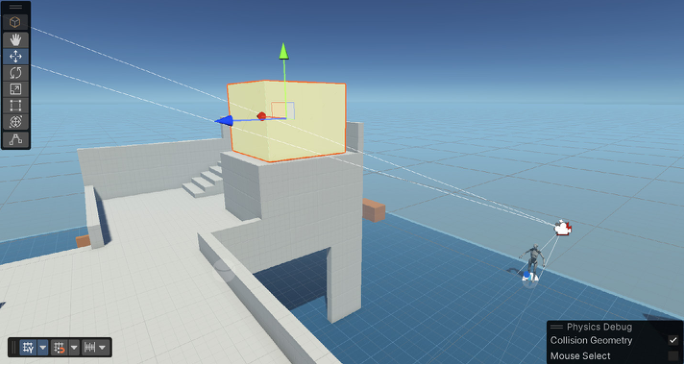
\includegraphics[width=0.76\linewidth]
    {../buku_ajar/chapters/13/figures/editor-fisika.png}}\par
\vspace{0.04cm}
\sumber{Level \emph{greyboxing} dengan bentuk batas ditampilkan panel
\emph{Physics Debug}. Kotak kuning adalah Collider, jauh lebih sederhana
daripada gambarnya.}
\begin{kotak}
Panel dibuka melalui \emph{Window} $\rightarrow$ \emph{Analysis} $\rightarrow$
\emph{Physics Debug}. Bila bentuk batas tidak tampak di tempat seharusnya,
penyebabnya hampir pasti letak atau ukuran Collider, bukan kode Anda.
\end{kotak}
\end{frame}

\begin{frame}{Urutan Penelusuran yang Disarankan}
\awalan{Empat langkah berikut disusun dari yang paling murah.}
\begin{enumerate}
  \item Periksa komponen pada \emph{Inspector}: apakah benda bergerak memiliki
        Rigidbody dan Collider, dan apakah Collider-nya ditandai trigger tanpa
        sengaja.
  \item Tampilkan bentuk batas melalui \emph{Physics Debug}, lalu periksa letak
        dan ukurannya.
  \item Periksa pengaturan fisika yang berkaitan dengan gejala:
        \emph{Gravity Scale}, \emph{Collision Detection}, dan
        \emph{Interpolate}.
  \item Baru periksa kode Anda; periksa lebih dahulu apakah Rigidbody digerakkan
        pada fungsi yang tepat.
\end{enumerate}
\vspace{0.10cm}
\begin{peringatan}
Pada blok Python masalah selalu berada pada kode Anda. Pada Unity, sebagian
besar masalah justru berada pada pengaturan komponen; menelusuri kode lebih
dahulu adalah kebiasaan lama yang perlu disesuaikan.
\end{peringatan}
\end{frame}

% ========================================================= bagian 6
\section{Kamera, Rasa Gerak, dan Penutup}
\sectionframe{06}{Kamera, Rasa Gerak, dan Penutup}
  {Mengikuti pemain, mengatur rasa, menutup Blok III}

\begin{frame}[fragile]{Kamera yang Mengikuti Pemain}
\begin{lstlisting}
void LateUpdate()
{
    Vector3 target = new Vector3(pemain.position.x, pemain.position.y,
                                 transform.position.z);
    transform.position = Vector3.Lerp(transform.position, target,
                                      followSpeed * Time.deltaTime);
}
\end{lstlisting}
\kodejelas{\texttt{LateUpdate} dipanggil setelah seluruh \texttt{Update} dan
\texttt{FixedUpdate} selesai, sehingga letak pemain pada bingkai itu sudah
pasti.}
\begin{itemize}
  \item \texttt{Vector3.Lerp} mengambil nilai antara dua letak menurut satu
        angka; kamera menyusul berangsur, bukan mengikuti dengan tepat.
  \item Nilai pengali yang kecil membuat kamera lebih lambat menyusul---salah
        satu pengatur rasa gerak yang paling berpengaruh.
\end{itemize}
\end{frame}

\begin{frame}{Mengatur Rasa Gerak}
\awalan{Rasa gerak permainan platformer sebagian besar ditentukan lima nilai,
dan seluruhnya dapat diatur tanpa mengubah kode.}
\begin{itemize}
  \item \textbf{Kecepatan mendatar} --- seberapa gesit pemain berpindah.
  \item \textbf{Kecepatan lompatan} --- menentukan tinggi lompatan.
  \item \textbf{\emph{Gravity Scale}} --- seberapa cepat pemain jatuh kembali;
        bersama kecepatan lompatan, ia menentukan lama pemain berada di udara.
  \item \textbf{Kelambatan kamera} --- seberapa jauh kamera tertinggal dari
        pemain.
  \item \textbf{Daerah pemeriksaan tanah} --- seberapa mudah pemain melompat,
        khususnya di tepi bongkahan.
\end{itemize}
\begin{kotak}
Kelima nilai itu seluruhnya pilihan perancang dan tidak satu pun berasal dari
perhitungan. Yang menentukan rasa permainan bukan tinggi lompatan itu sendiri,
melainkan perbandingan antara nilai-nilainya.
\end{kotak}
\end{frame}

\begin{frame}{Menutup Blok III}
\awalan{Bab ini menutup CPMK 3: kemampuan menggunakan \emph{game engine} untuk
membangun level.}
{\scriptsize
\renewcommand{\arraystretch}{1.12}
\begin{tabularx}{\textwidth}{@{}>{\raggedright\arraybackslash}p{3.6cm}
    >{\raggedright\arraybackslash}p{1.8cm}
    >{\raggedright\arraybackslash}X@{}}
\toprule
\textbf{Perkakas} & \textbf{Dibahas pada} & \textbf{Kegunaan} \\
\midrule
Antarmuka dan penyusunan benda & Bab XII &
  Mengelola \emph{project}, \emph{scene}, dan benda beserta komponennya. \\
\addlinespace
Skrip dan urutan pemanggilannya & Bab XII &
  Menempatkan pekerjaan pada fungsi yang tepat. \\
\addlinespace
Penyusunan level & Bab XIII &
  Menyusun ruang permainan secara \emph{greyboxing} dan dengan \emph{tilemap}. \\
\addlinespace
Fisika dan tabrakan & Bab XIII &
  Mengonfigurasi Collider, Rigidbody, dan trigger, serta memperbaiki
  masalahnya. \\
\bottomrule
\end{tabularx}}
\vspace{0.14cm}
\begin{kotak}
Bab XIV sampai Bab XVI melengkapi level ini dengan aset visual, antarmuka,
audio, dan pengujian prototipe. Seluruhnya berpijak pada level yang baru saja
Anda bangun.
\end{kotak}
\end{frame}

% --------------------------------------------------------- aktivitas
\begin{frame}{Aktivitas di Kelas \textperiodcentered\ Praktikum 10}
\setbeamerfont{itemize/enumerate body}{size=\scriptsize}
\awalan{Pengalaman belajar minggu 12 pada RPS, dikerjakan berurutan di kelas lalu
diselesaikan di rumah.}
\begin{enumerate}
  \item Susun level secara \emph{greyboxing}: lantai dari Tilemap atau balok,
        sekurang-kurangnya tiga bongkahan pada ketinggian berbeda, dan dua
        dinding.
  \item Tetapkan ukurannya lebih dahulu---tinggi lompatan, lebar celah, tinggi
        bongkahan---lalu sisakan kelonggaran sepuluh sampai dua puluh persen.
  \item Tambahkan pemain: \texttt{Rigidbody2D}, \texttt{Capsule Collider 2D},
        dan skrip \texttt{KontrolPemain}; kunci putarannya melalui
        \emph{Constraints}.
  \item Atur pemeriksaan tanah: benda kosong \texttt{groundCheck} di bawah kaki,
        \emph{layer} tanah, dan pastikan lingkarannya tampak pada panel
        \emph{Scene}.
  \item Jalankan dan mainkan; bila ada yang tidak sesuai, telusuri menurut
        urutan pada Bagian 5 dan catat hasilnya.
  \item Tambahkan daerah trigger di ujung level, tempel \texttt{TriggerPintu},
        periksa panel \emph{Console}, lalu tambahkan kamera yang mengikuti.
\end{enumerate}
\vspace{0.08cm}
{\footnotesize\color{ubAccent}\itshape Rincian lengkap: Praktikum 10 pada
Bab XIII buku ajar. Kumpulkan melalui repositori Git pribadi.}
\end{frame}

% --------------------------------------------------------- rangkuman
\begin{frame}{Rangkuman}
\setbeamerfont{itemize/enumerate body}{size=\scriptsize}
\begin{itemize}
  \item \emph{Greyboxing} menguji mekanik sebelum aset dibuat; \emph{tilemap}
        menyusun petak berulang dan cukup memerlukan satu Collider.
  \item Ukuran level---tinggi lompatan, lebar celah, tinggi bongkahan---
        ditetapkan lebih dahulu dan saling bergantung.
  \item Benda diam cukup Collider; benda bergerak memerlukan Collider dan
        Rigidbody. Tiga tipenya: \emph{dynamic}, \emph{kinematic},
        \emph{static}.
  \item \emph{Trigger volume} tidak menghalangi; syaratnya tanda
        \emph{Is Trigger}, keberadaan Rigidbody, dan \emph{layer} yang saling
        diperiksa.
  \item Masukan dibaca pada \texttt{Update}, gerak dan pemeriksaan tanah
        dikerjakan pada \texttt{FixedUpdate}; kamera dipindahkan pada
        \texttt{LateUpdate}.
  \item Empat masalah fisika---bergetar, menembus Collider, jatuh tanpa henti,
        tersangkut---ditelusuri dari komponen, bentuk batas, pengaturan, baru
        kode.
\end{itemize}
\end{frame}

% --------------------------------------------------------- cek
\begin{frame}{Cek Pemahaman}
\begin{enumerate}
  \item Mengapa benda diam tidak perlu diberi Rigidbody, dan apa akibatnya
        apabila tetap diberikan?
  \item Sebuah benda bergerak 30 satuan per detik, lantainya tebal 0,1 satuan,
        dan langkah fisika 0,02 detik. Tentukan apakah benda itu dapat menembus
        lantai, beserta perhitungannya.
  \item Mengapa kamera dipindahkan pada \texttt{LateUpdate}, bukan pada
        \texttt{Update}?
\end{enumerate}
\vspace{0.35cm}
{\footnotesize\color{ubMuted}\itshape Jawab tanpa membuka catatan, lalu
bandingkan dengan pasangan di sebelah Anda.}
\end{frame}

% --------------------------------------------------------- penutup
\penutup{Tugas Praktikum 10}
  {Materi 12 \textperiodcentered\ Impor Aset Visual, Animasi, dan UI Dasar:
   \emph{sprite sheet} dan \emph{Animator} menggantikan \emph{placeholder}
   \emph{greybox}, lalu \emph{Canvas} UI menampilkan skor dan nyawa.}

\end{document}
